\begin{scanpage}{0111}{94}
\noindent\begin{minipage}[t]{.31\linewidth}\vspace{0pt}\centering
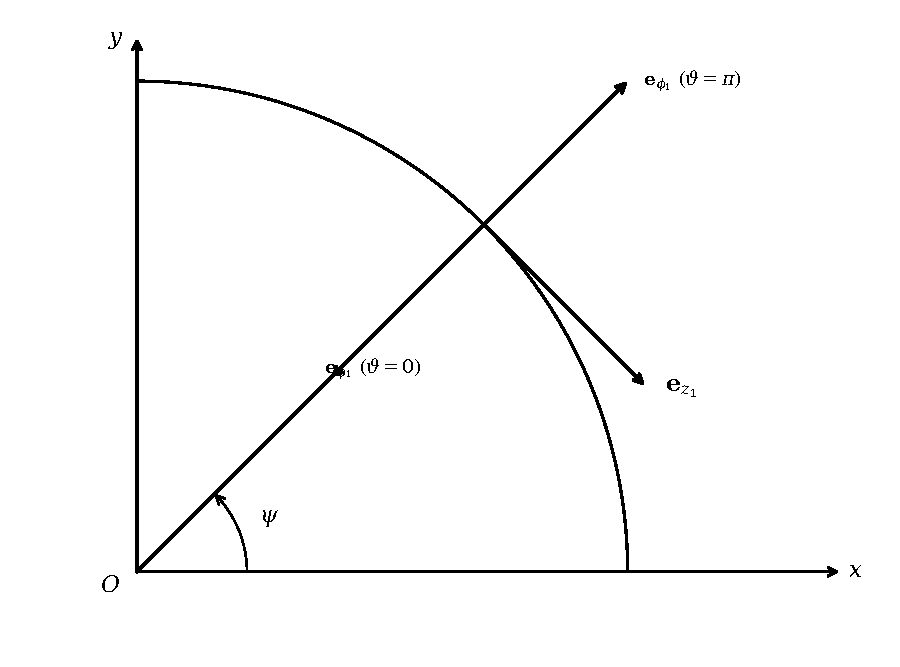
\includegraphics[width=\linewidth]{images/recreated/b-0111-fig30.pdf}

Figure 30. The relative orientation of the unit vectors $\mathbf e_{\phi_1}$ and $\mathbf e_{z_1}$ in the cases $\vartheta=0$ and $\vartheta=\pi$.
\end{minipage}\hfill\begin{minipage}[t]{.65\linewidth}\vspace{0pt}
\[\left.\begin{aligned}A_x&=\frac a{ik2\pi}\frac{e^{ikr}}r\int_0^{2\pi}[f^1E_{0z_1}(\psi)\sin\psi\\&\quad-g^1H_{0z_1}(\psi)\cos\psi]d\psi,\\A_y&=-\frac a{ik2\pi}\frac{e^{ikr}}r\int_0^{2\pi}[f^1E_{0z_1}(\psi)\cos\psi\\&\quad+g^1H_{0z_1}(\psi)\sin\psi]d\psi\end{aligned}\right\}\tag{16.15}\]
with $\vartheta=0$

and
\[\left.\begin{aligned}A_x&=\frac a{ik2\pi}\frac{e^{ikr}}r\int_0^{2\pi}[f^1E_{0z_1}(\psi)\sin\psi\\&\quad+g^1H_{0z_1}(\psi)\cos\psi]d\psi,\\A_y&=-\frac a{ik2\pi}\frac{e^{ikr}}r\int_0^{2\pi}[f^1E_{0z_1}(\psi)\cos\psi\\&\quad-g^1H_{0z_1}(\psi)\sin\psi]d\psi\end{aligned}\right\}\tag{16.16}\]
with $\vartheta=\pi$.
\end{minipage}\par\medskip

Furthermore, let the plane wave be polarized in such a way that $\mathbf E_0\parallel Ox$. Then
\[E_{0z_1}(\psi)=E_{0x}\sin\psi,\quad H_{0z_1}(\psi)=-E_{0x}\cos\psi.\tag{16.17}\]
Considering these relationships and substituting Expressions (16.15) and (16.16) into Equations (16.02) and (16.03), we find the field from the nonuniform part of the current which is caused by the circular discontinuity of the conical surface
\[\left.\begin{aligned}E_x=H_y&=\frac{aE_{0x}}2(f^1+g^1)\frac{e^{ikr}}r,\\E_y=H_x&=0\end{aligned}\right\}\quad\text{with }\vartheta=0\tag{16.18}\]
and
\[\left.\begin{aligned}E_x=-H_y&=\frac{aE_{0x}}2(f^1-g^1)\frac{e^{ikr}}r,\\E_y=H_x&=0\end{aligned}\right\}\quad\text{with }\vartheta=\pi.\tag{16.19}\]
Equation (16.18) is applicable for the values $0<\omega<\frac\pi2$, $\omega<\Theta\leq\pi$, and Equation (16.19) for the values $0<\omega\leq\frac\pi2$, $0<\Theta\leq\pi$. In the case of a
\end{scanpage}
